\section {Databases}

For the database we had two subjects to study:
\begin{itemize}
        \item Databases for archival purposes
        \item Databases for storing files
    \end{itemize}

\subsection {Archival Database}

So taking the first one, we had to study performance to cost of three solutions and their scalability:

    \begin{itemize}
        \item RDS (SQL)
        \item DynamoDB (NoSQL)
        \item Aurora (SQL)
    \end{itemize}

As all three were AWS solutions, the performance of each was pretty much the same,
and as the database was going to be used for archival it relied less on having a
high throughput and more on how much storage costs.
So we only relied on the cost of the solution, how easy is it to maintain.

So going off by cost first Aurora was the most expensive, with no value added to the problem we'll be solving with it.

So that left us with two options:

    \begin{itemize}
        \item RDS (SQL)
        \item DynamoDB (NoSQL)
    \end{itemize}

We dived into the RDS solution, and it was a bit of a challenge to get it to scale,
in terms of storage compared to DynamoDB which offered autoscaling options and variable
throughput for high load time which could fit the needs of archival as it could take 
higher input in the daily backup process, than the rest of the day.
And for the output there wasn't much to be gained, for neither of the solutions as it was
a rare process that wouldn't be used alot only on demand by the user.

Going to studying the cost, the primary tool that was used for that is the AWS Cost Calculator, which gives rather good indicators to approximate the charges.

\textbf{Case study: }

For the data we used the following:
- 200 Entries per site.
- 500 Site.
- 2 KB per entry.

Site represents the factories and the entries represents the trucks.

So with those inital values, we came to the following results:
- Daily storage of 200 MB or monthly of 6 GB that increments after the period passes.
- 3000000 writes / month
- 100000 reads / month

the reads were just second guessed as there was no significant data about it, 
other than it will be a low read database.

So for the calculations, for RDS we used the following options:
- Instance db.t3.large (vCPU: 2 Memory: 8 GB)
- Instance reserver for one year 
- Single-AZ (1 node)
- 6 GB storage incremented monthly
- 6 GB backup incremented monthly

which resulted in the yearly cost of \$1185.769

For DynamoDB, we used the following options:
- Standard-Infrequent Access (Reduces cost of storage)
- 3 Mil writes per month
- 100K reads per month
- 6 GB storage incremented monthly
- 6 GB backup incremented monthly

Which came down to the cost of \$236.00 per year.

As we can notice the RDS cost was much higher than DynamoDB,
so we decided to use DynamoDB as it was cheaper, and also had
better maintenance options offered by AWS as it's a fully hosted
service.

Lastly, the only missing part was integration within the back-end which went on different steps.

First we had to create a service on the Spring Back-end that took on the handling of the communication layer between the DB and the back taking on mulitple functionalities such as:

    \begin{itemize}
        \item Creating - delete tables
        \item Creating indexes to allow fast access to the data
        \item Adding - deletting data
        \item Finding data using specific fields
    \end{itemize}

Then implementation of unit tests for the service to ensure that it's working as intended,
it had taken on the following tests:

    \begin{itemize}
        \item Create table for tests with required indexes
        \item Adding data to table, and then finding it
        \item Adding data to table, and find it by date
        \item Adding data to table, and find it by different keys
        \item Cleaning up the table
    \end{itemize}

Finally the creation of the tables and their indexes was automated, to allow for the
reproduction of the same environment for the data we had during testing, and in the 
dev environment.

\newpage

Final the archival process was as follows:
\begin{figure}[!htbp]
    \centering
    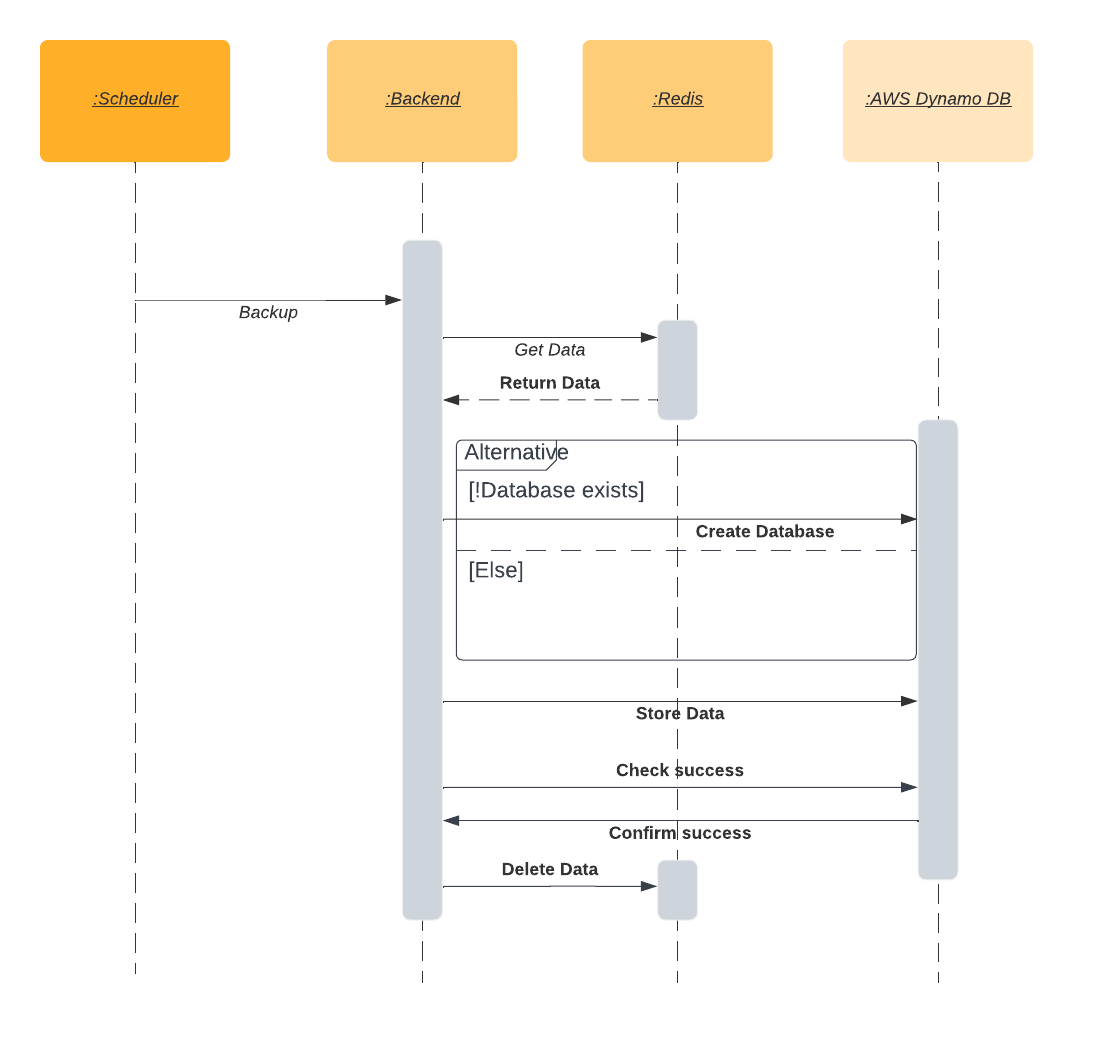
\includegraphics[width=\textwidth]{images/archival_backup.png} 
    \caption{\footnotesize{Archival Cronjob}}
    \label{fig:archival_backup}
\end{figure}

The cronjob for handling the archival had a pretty simple process, 
it would take the data each day at 00:00 and archive it from the redis
database to the DynamoDB while checking that everything was successfully archived
before cleaning the data from Redis.

\subsection {File storage Database}

For this second database, that is more opted to be used for the storage of files.
The solution was already known, and was the Amazon S3 service.

The file storage database was used for the following:

    \begin{itemize}
        \item Storing site configuration files
        \item Storing client files
    \end{itemize}

The storage was pretty simple, it was just a bucket with a specific folder structure.
So for the first case it was a folder for each site,
and for the second it was a folder for each client which was handled with the archival
cronjob as these files were related to the data from the trucks that have been handled
during the day.

For the tests we used the following:

    \begin{itemize}
        \item Creating a bucket
        \item Creating a folder structure
        \item Adding data to the bucket and finding it
        \item Deleting data from the bucket
        \item Deleting the bucket
    \end{itemize}

For the creation of the bucket it was made such as it's done automatically once the
server started in case it doesn't exist.

So that we can reproduce the same bucket that there was in the dev environment and during
the  tests.

\section {Security and Authentication}

\subsection {Ratelimiting}

Ratelimiting was one interesting aspect for security, as it's a way to prevent the
server from being flooded with requests. As it could stop DOS attacks, brute force
attacks, and any other kind of attack that would require sending lot of request from 
the same IP or same user.

For the ratelimiting, as we were using already a Spring backend we had a couple options
to choose from the first one was Bucket4j, which is a ratelimiter that relies on having
a bucket for each key, the key could be a user, IP address, APi key ...

The second option was to use Resilience4j, which relied on a circuit breaker to
handle the ratelimiting but it was not easy to implement for the case of a distributed
backend, as it relied heavily on single machines threads and not clusters.

So we went with the former, which was implemented as a filter in front of the API gateway
in the Spring backend.

\begin{figure}[!htbp]
    \centering
    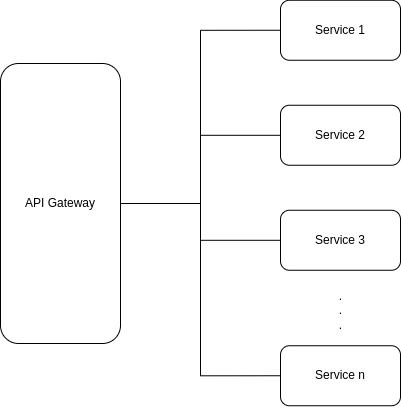
\includegraphics[width=0.5\textwidth]{images/ratelimiting.png} 
    \caption{\footnotesize{Bucket4j}}
    \label{fig:bucket4j}
\end{figure}


As seen in the figure \ref{fig:bucket4j}, that's the basic handling of services within the
Java Spring backend, so the ratelimiting was implemented in the API gateway such as to
stop any coming requests before they can have access to any service.

The ratelimiting was handled in two ways, the first was to have a bucket for each user,
and the second was to have a bucket for each IP address.

Ratelimiting the user was specifically setup for handling the private endpoints and that
was able to be modified by the admin to allow for more or less requests per second
depending on the user, and the ratelimiting the IP address was setup for the public API.

And lastly there was the ratelimiting for the login, which was individually handled for
the purpose of limiting the number of login attempts per minute to avoid possibility
of a dictionnary attack.

\subsection {Authentication}

TODO

\newpage

\section {Containerization and Deployment}

Before we dive in into the specifics, we first will showcase the final architecture in the ECS, which is below:

\begin{figure}[!htbp]
    \centering
    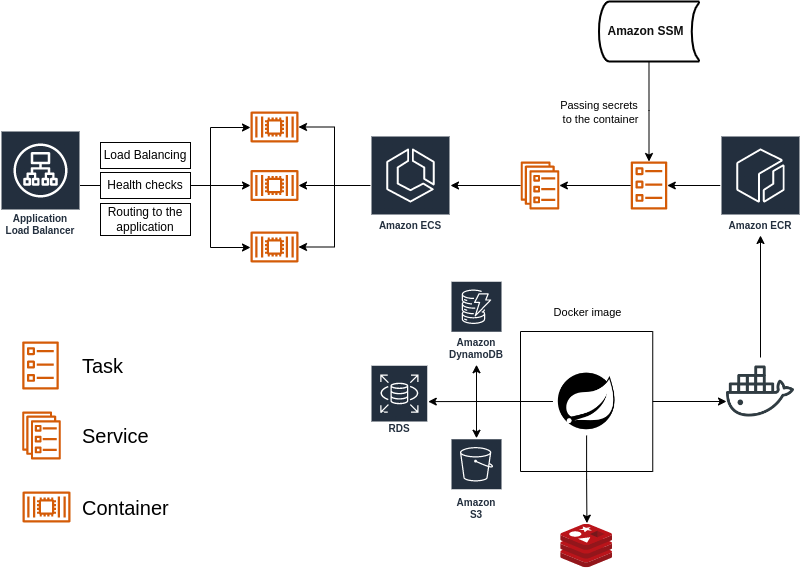
\includegraphics[width=\textwidth]{images/ECS}
    \caption{\footnotesize{ECS Architecture}}
    \label{fig:ECSArch}
\end{figure}

Task: the component which takes care of running the containers.

Service: the component which manages the tasks.

Container: the image that is running on the task.

\subsection {ECS Containerization and secrets}

The ECS solution was a bit of a challenge to get it to work,
as it was a containerized solution, and not a native one.
So the first step was to containerize the solution, and have a safe image 
that doesn't expose any secrets or environment variables.

In the docker way, we can just pass them through the command line,
and the solution will run perfectly.

But here relied a problem that was the ECS solution, it didn't have a simple
way to feed it the credentials, environment variables neither files, so we had to opt
for using the SSM or Secrets Manager
which is yet another hosted solution to store strings as secrets, and then those could be 
passed to the ECS services.

With the Secrets Manager, for the strings secrets it was a simple writing / reading process
to store and retrieve the secrets. But for the files it was a bit more complicated, there
wasn't a direct way to do that.

Finally we came up with the following solution, which is as follows:

\begin{itemize}
    \item Serialize the content of the file into a base64 string
    \item Store the base64 string in the SSM
    \item Pass the SSM secret to the ECS service
    \item Retrieve the secret from the SSM as a environment variable
    \item Decode the base64 string
    \item Store the deserialized base64 in a file in the container
    \item Point an environment variable to the file
\end{itemize}

As such we managed to pass aws credentials, google credentials and Redis Labs credentials.

\subsection {Load Balancer and routing}

As shown in the ECS Architecture, we had a load balancer in front of the running tasks, which has four main goals:

\begin{itemize}
    \item To take care of the incoming traffic from the client side
    \item To ensure that the traffic distributed evenly
    \item To ensure that the tasks are healthy
    \item To ensure that the tasks are not overloaded and manage it's scalability.
\end{itemize}

\begin{figure}[!htbp]
    \centering
    \includegraphics[width=\textwidth]{images/loadBalancer.png}
    \caption{\footnotesize{Load Balancer Interaction with the backend}}
    \label{fig:loadbalancer}
\end{figure}

So the load balancer is as shown in figure \ref{fig:loadbalancer}, it took traffic from
port 80 where it had an exposed dns link, then it routed it through a VPS to the
containers that are exposing post 8080 in their local network, having healthchecks
done on the endpoint /actuator/health .

\newpage

With that set in place, we had pretty much everything setup to start testing for the
load handling by the ecs to check for the health of the containers and the measures
to be set to ensure that the auto scaling is setup with the right parameters.

So first, we written scripts that did kind of overload the server with the requests,
asynchronously deploy the containers and check monitoring metrics.


The script worked as follows:

\begin{figure}[!htbp]
    \centering
    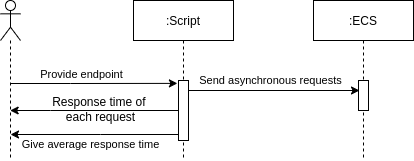
\includegraphics[width=0.7\textwidth]{images/scriptdos.png}
    \caption{\footnotesize{Load Test Script}}
    \label{fig:loadtest}
\end{figure}

So firstly it took the endpoint to be hit, in case it was a private endpoint you'd need to
provide the credentials to. Then put in place the number of requests to be sent and
finally run it.

Once it started running it was a simple case of sending requests asynchronously in fibers
or virtual threads, and then printing the response time of each request, as such we could
monitor the handling time of the requests being affected by the load of requests.

Thus it we could find the right parameters for the auto scaling, based on the number of
requests being sent per second, which at the time of tests was around 1000 request per
second without the response time being affected.

And as most the back-end services relying heavily on the memory, we ensured to put a 70\%
memory usage limit on the containers before spawning new instances to handle the load, in
case of autoscaling by memory.

\subsection{Deployment}

Finally after testing everything, and having deployed one ECS service succesfully, we had
to automate the deployment process, so that we could handle new versions and code update
without much effort.

This came in the form of a gradle task, which was as follows:

    \begin{figure}[!htbp]
        \centering
        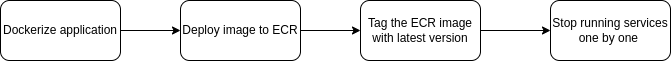
\includegraphics[width=\textwidth]{images/gradle.png}
        \caption{\footnotesize{Gradle Task}}
        \label{fig:gradle}
    \end{figure}

The dockerization part of the gradle task was handled using a third party plugin,
then the deployment to ECR is done using the AWS CLI, by linking the ECR to docker,
then pushing the image is automatically uploaded to ECR.
Once this is done, the ECS service has to handle the update of the image, 
and this was done through a bash script that took in charge of getting a list 
of the running tasks, then stopping one of them, and wait for a new one to spawn 
such as to avoid down time during the update of the service.

\section {Refactoring and Improvements}

\subsection {Adding a user management system}

The old system didn't have a user management system, as it relied on the site being the
user so there wasn't really users to manage. So we had to integrate users within the system
then add a way to manage them, and this was done by migrating the site from being the user
to being an entity that could be managed by users who have the right to do so.
And that required rework through the majority of the backend as this architecture was
relied on by all the backend services and controller and also frontend.

So we had to change this architecture to be able to manage users and their roles, but also
keep the old behaviour the same.

TODO: Add class diagram before and after (Couldn't do it now because we migrated directly without using diagrams)
